\subsection{Laying pipes in the clouds}\label{sec:rate-control}

\begin{figure*}[!t]
  \centering
    \begin{subfigure}{0.65\columnwidth}
  \centering
  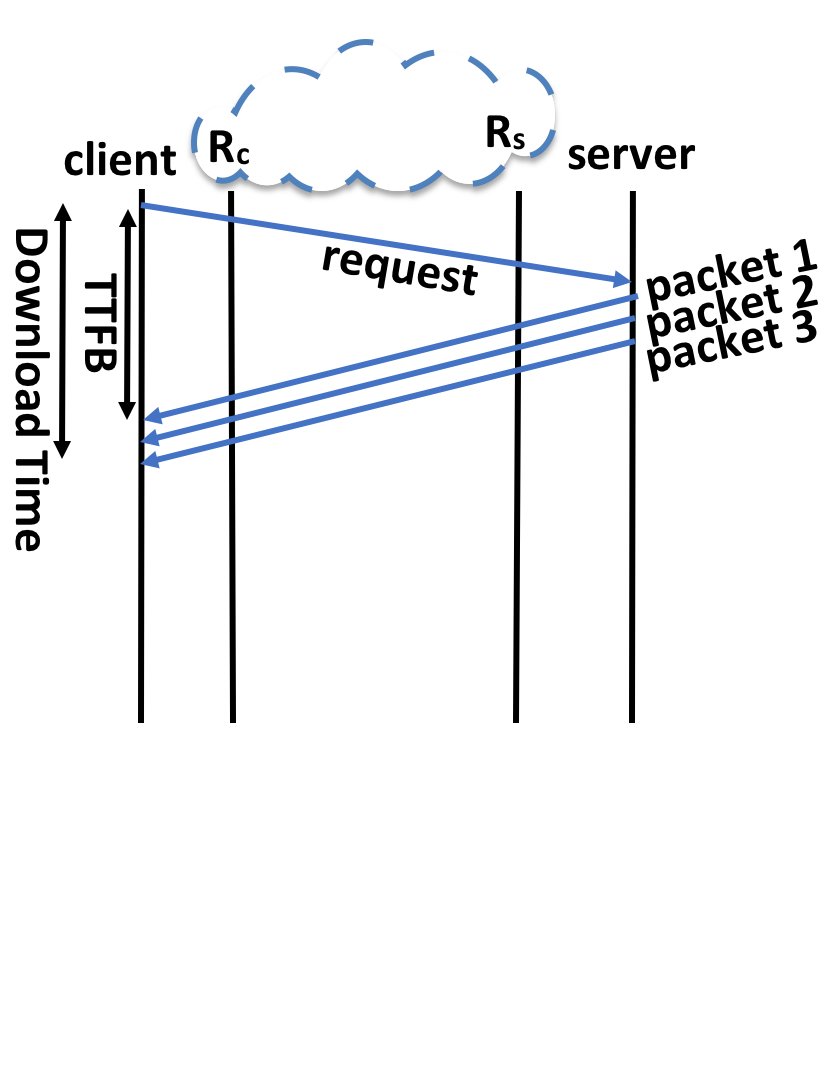
\includegraphics[width=\columnwidth]{figures/ideal.png}
    \caption{Ideal protocol-free transmission.}
    \label{fig:ideal}
\end{subfigure}    \centering
\begin{subfigure}{0.65\columnwidth}
  \centering
  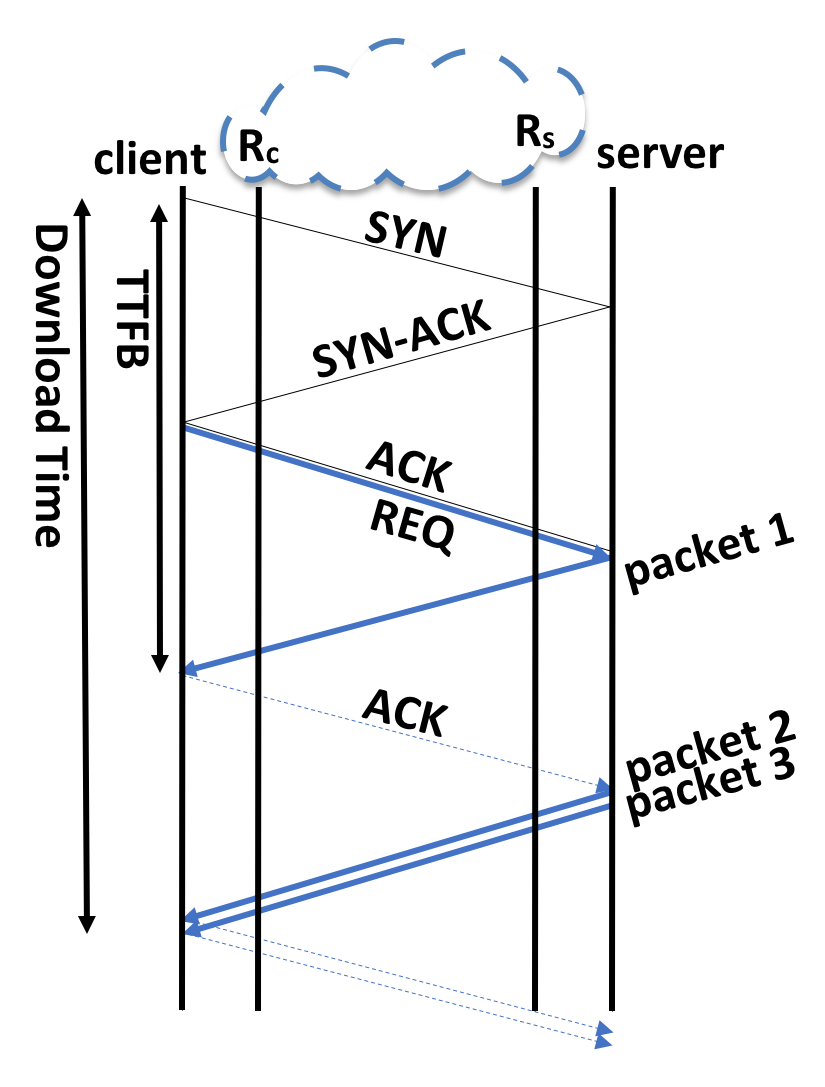
\includegraphics[width=\columnwidth]{figures/e2e.png}
    \caption{End-to-end (no split) transmission.} \label{fig:e2e}
\end{subfigure}    \centering
\begin{subfigure}{0.65\columnwidth}
  \centering
  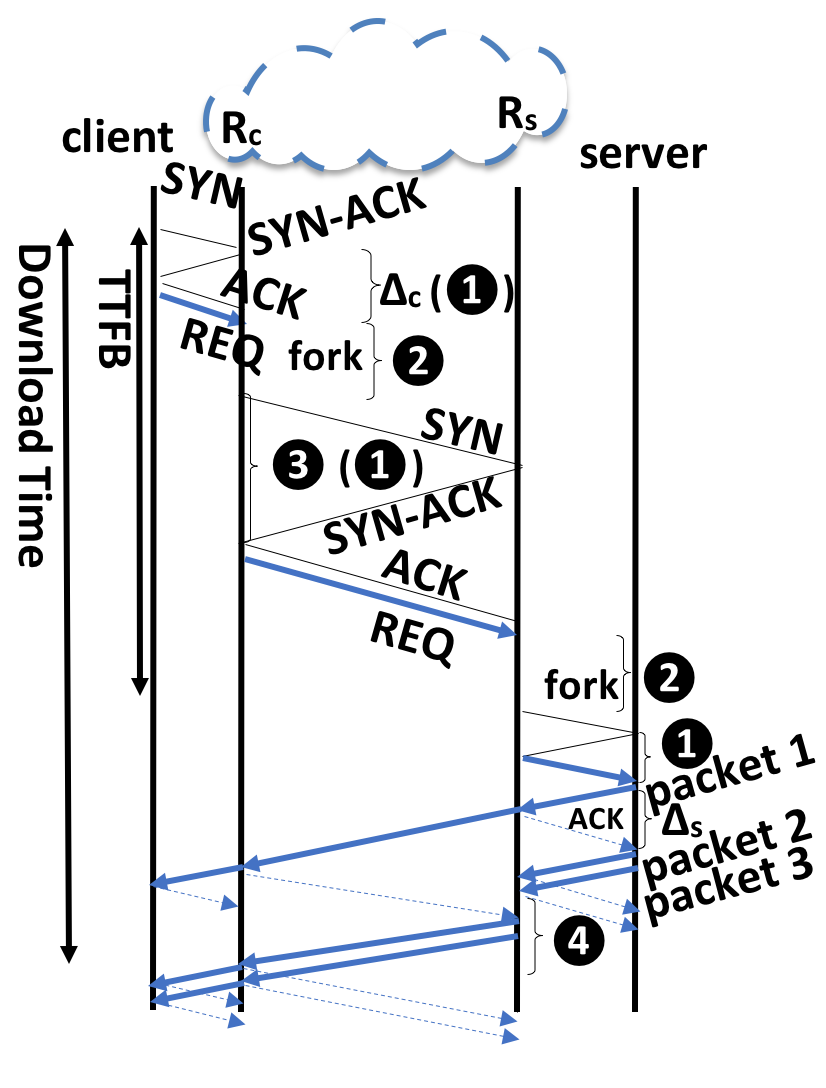
\includegraphics[width=\columnwidth,clip]{figures/split.png}
    \caption{Simple TCP split, on both \rc and \rs \AB{is (4) correctly marked in the drawing?}} \label{fig:baseline}
\end{subfigure}

    \caption{Illustrated comparison of the considered baseline data transmission methods.}
\end{figure*}

\begin{figure*}[!t]
  \centering
    \begin{subfigure}{0.75\columnwidth}
  \centering
  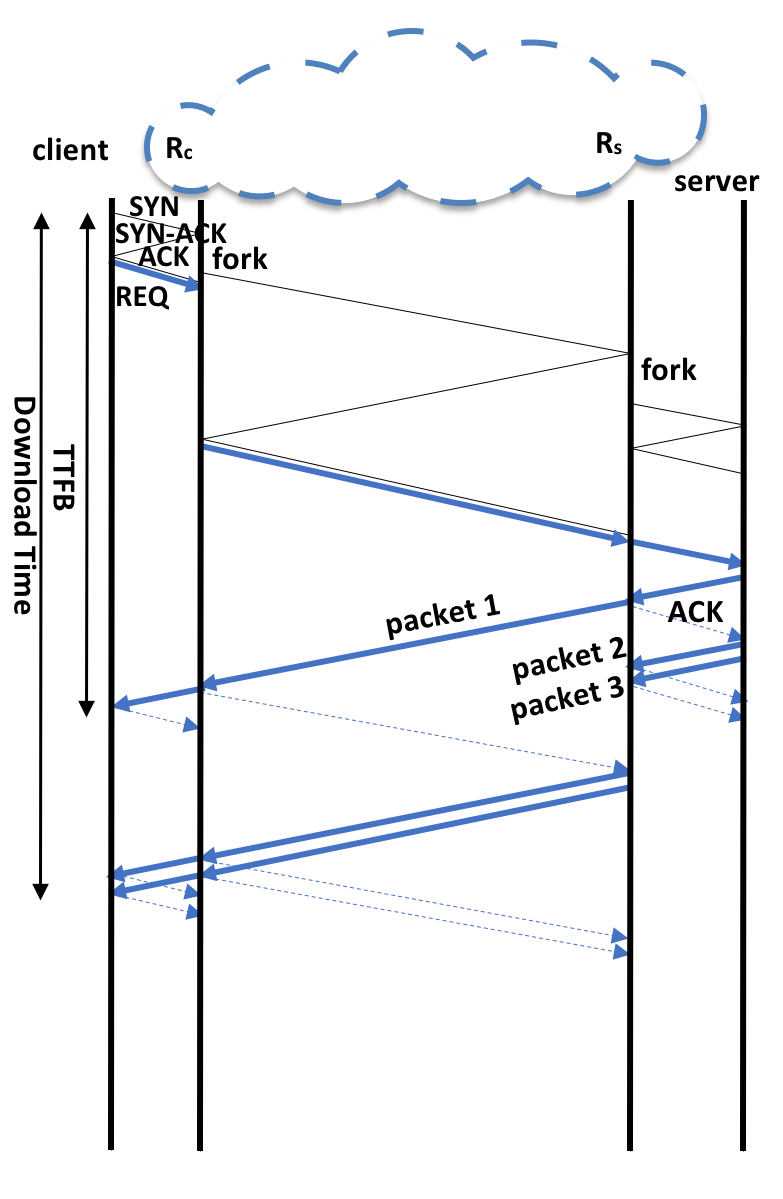
\includegraphics[width=\columnwidth]{figures/early-syn.png}
    \caption{Early-SYN.}
    \label{fig:early-syn}
\end{subfigure}    \centering
\begin{subfigure}{0.75\columnwidth}
  \centering
  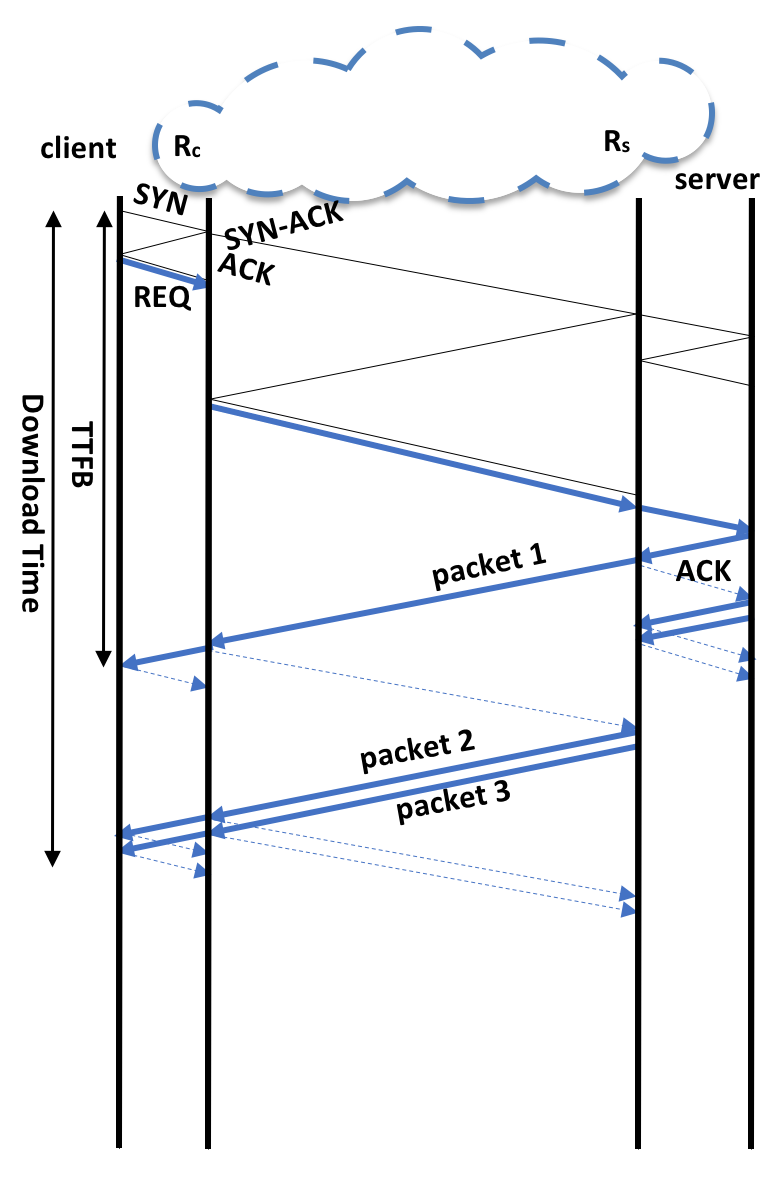
\includegraphics[width=\columnwidth]{figures/thread.png}
    \caption{Thread pool.} \label{fig:thread-pool}
\end{subfigure}    \centering
\begin{subfigure}{0.75\columnwidth}
  \centering
  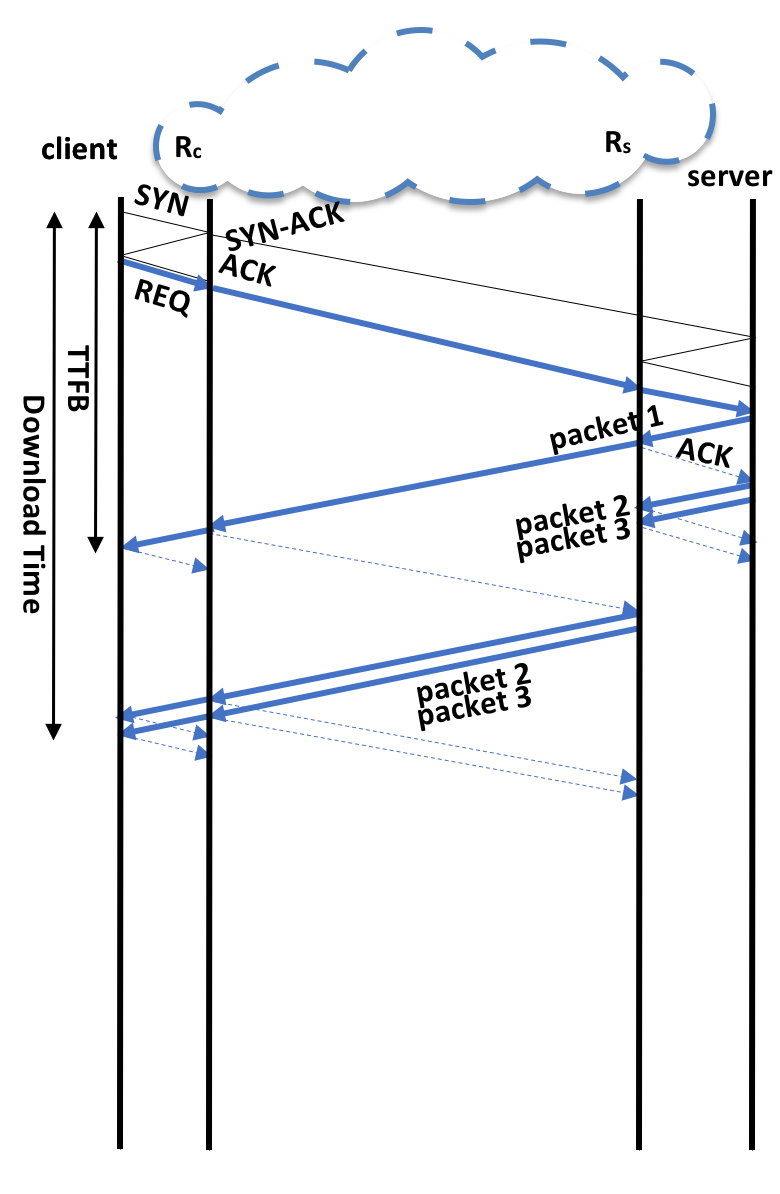
\includegraphics[width=\columnwidth]{figures/connection.png}
    \caption{Connection pool.} \label{fig:connection-pool}
\end{subfigure}     \centering
\begin{subfigure}{0.75\columnwidth}
  \centering
  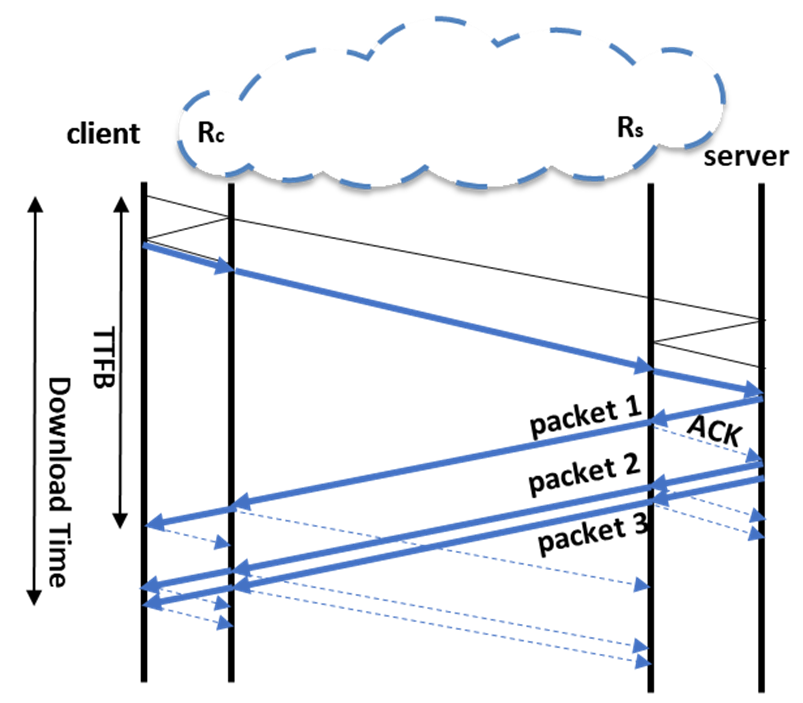
\includegraphics[width=\columnwidth]{figures/turbo.png}
    \caption{Turbo-Start TCP.\AB{is it me, or are the lines thinner in this figure?}} \label{fig:turbo-start-tcp}
\end{subfigure}

    \caption{\oursys successive implementation improvements \AB{maybe spread the figures a bit on the x axis?}}
    \label{fig:oursys-improvements}
\end{figure*}

%\begin{figure}[t]
%  \centering
%\begin{subfigure}{0.7\columnwidth}
%  \centering
%  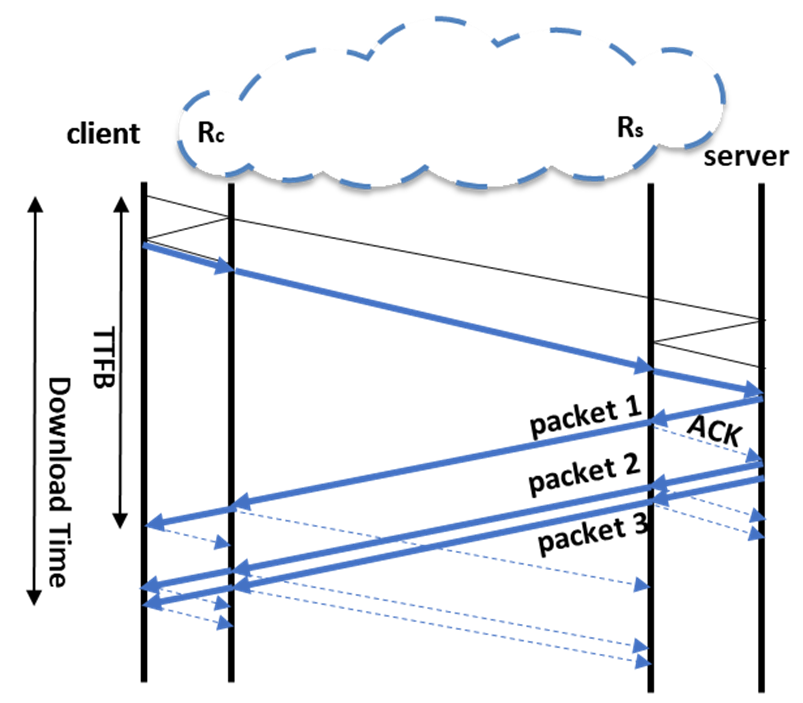
\includegraphics[width=\columnwidth]{figures/turbo.png}
%    \caption{Turbo-Start TCP.} \label{fig:turbo-start-tcp}
%\end{subfigure}
%
%    \caption{Illustrated comparison of the considered baseline data transmission methods.}
%\end{figure}

%\T{Congestion-less control?} The cloud provides an auto-scaling networking infrastructure with links of virtually-infinite capacity. Like others~\cite{haq2017measuring}, we find that in-cloud paths provide more predictable results than the public Internet, with an order of magnitude lower loss rate. As a result, flows in the cloud will rarely ever encounter congestion. This compels us to rethink the role of congestion control in the cloud. In light of the near-absence of congestion, we essentially want a simple high-rate sending protocol capable of dealing with the very rare loss events, without necessarily backing off. Even flow control is not necessarily needed within the cloud, as clouds can increasingly provide an elastic memory infrastructure~\cite{hotadd,baloon} that can quickly adapt to any receive-buffer temporary load. 

%\T{Ideal pipe.} 
The cloud provides an auto-scaling networking infrastructure with links of virtually-infinite capacity. Like others~\cite{haq2017measuring}, we find that in-cloud paths provide more predictable results than the public Internet, with an order of magnitude lower loss rate. As a result, flows in the cloud will rarely ever encounter congestion\AB{I'm not sure I follow - congestion is not the result of loss rate. It's usually the other way around. Perhaps you'd like to put this sentence right after the ``virtually-infinite'' sentence and then quote \cite{haq2017measuring} as evidence}. Given the favorable conditions in the cloud, we wonder if we could facilitate an ideal transmission. \autoref{fig:ideal} illustrates our fundamental model of an ideal transmission. Importantly, this model reflects a protocol-free, theoretical ideal transmission.
In this example, we suppose;\AB{why the semicolon?} that the client requests three MSS-sized packets using HTTP over TCP, that the initial TCP window size is one MSS, and that there are no losses.
\AB{Did you mean to present the following as a list?}
 \textit{Ideal (\autoref{fig:ideal}):} In an ideal clean-slate world, the request for packets would go through the \relays\AB{I don't think a reader who is unfamiliar with our previous paper would understand why we have relays at all, or why we have two. It is also not clear at this point what the location of \rc and \rs is, or should be, and why.}\footnote{The two \relays are depicted as \rc and \rs in all figures} directly.  \AB{Something missing here? (It's an incomplete sentence...)} triggering the transmission of all response packets. The time-to-first-byte (TTFB) is just one round-trip time (RTT), the lowest possible TTFB. \AB{I'm not sure it is clear that at this point we are disregarding any TCP-related overhead, such as its 3-way handshake.}\\
Unfortunately, the classical end-to-end data transfer shown in \autoref{fig:e2e}, falls short of this ideal model.
 \textit{Real (\autoref{fig:e2e}):} End-to-end TCP transmission based on HTTP over TCP \AB{This sounds weird - TCP transmission based on HTTP over TCP?}, first requires the establishment of an end-to-end connection, adding one RTT to the ideal finish time. Waiting one RTT for the first ACK further delays the download\AB{Did you mean the ACK sent from the client on the first data packet from the server, and that this is due to TCP's cwnd behavior? It wasn't clear when I read this.}.\\ 
\AB{Perhaps first mention that now you are talking about TCP split...}In addition to the delays caused by TCP, each "stop"\AB{?} on one of the \relays also introduces additional delays. These delays are shown in \autoref{fig:baseline}.
\textit{Split (\autoref{fig:baseline}): } The basic TCP split decreases the ACK times\AB{What is ``ACK time''} and thus speeds up download time for larger files. But a naive implementation also introduces additional overheads which we discuss in section ~\ref{sec:approx}\AB{It seems weird to me to delay the description of the various delays to the next section. Is there a reason not to describe these here?}. These overheads explain why the naive implementation is detrimental for small files.  (Figure~\ref{fig:oursys-improvements}) \AB{why is this here?}. We show how to address the delays marked (1)-(4), but are left with delays $\Delta_c$ and $\Delta_s$ on the client and server sides, respectively. \AB{maybe add that this is the reason one would want to place \rc and \rs as close as possible to the client and server, respectively.}

\section{Approximating the Ideal Pipe}\label{sec:approx}

To approximate the ideal data transmission model, we introduce \textit{\oursys}.
The goal of \oursys is to provide efficient, delay-free\AB{It's not delay-free...} TCP optimization;\AB{I don't think ``;'' is called for here.} while utilizing commodity VMs and standard programming APIs. This is done by incorporating four improvements to the naive TCP split\AB{What do you refer to as ``naive TCP split''? Our brand of user-space TCP split? Any user-space TCP split? One based on Nginx? One that does not include any of the optimizations we later discuss?}. These improvements are illustrated in Figure~\ref{fig:oursys-improvements}. Together, these four components eliminate the delays marked (1)-(4) in Figure~\ref{fig:baseline}\AB{you have a very similar sentence in the previous paragraph}. We discuss the implementation details in Section~\ref{sec:design}.

%.  . Turbo-Start TCP eliminates delay (4). The two last delays (marked as ``?'' in Figure~\ref{fig:baseline}) that need be removed are delays $\Delta_c$ and $\Delta_s$ on the client and server sides, respectively. As both depend on the client and server parameters, are beyond our control.

%\oursys incorporates four improvements to the baseline strategy of Section~\ref{x}, illustrated in Figure~\ref{fig:baseline}. Together, these four improvements eliminate the delays marked (1)-(4) in \ref{fig:oursys-improvements}. We next elaborate on each of the four improvements. We discuss the many implementation details involved in realizing \oursys in Section~\ref{sec:design}.

\T{Improvement 1: Early SYN.} \xspace Figure ~\ref{fig:early-syn}. In early SYN~\cite{ladiwala,siracusano2016miniproxy}, a SYN packet is sent to the next-hop server as soon as the SYN packet arrives. This is done without waiting for the three-way handshake to complete. \oursys captures this first SYN packet and triggers the start of a new connection. This allows the proxy to establish the two legs of a split connection in parallel. Using \textit{Early-SYN}, we can remove SYN-ACK and ACK delays, marked as (1) in Figure~\ref{fig:baseline}.
While the notion of creating the two legs of the connection in parallel is not new, ours is the first to use standard Linux utilities.

\T{Improvement 2: Thread pool.}             
The creation of new processes or threads for each new split connection is \\time-consuming and adds greatly to the connection jitter. Some outliers may take tens of milliseconds, greatly hurting performance. For small files/objects, this jitter may even nullify the benefit of \oursys. To mitigate this problem, we create a pool of reusable threads. These are sleeping threads, awaiting to accept new tasks. Using a \textit{thread pool} removes the delays marked as (2) in Figure ~\ref{fig:baseline}. \AB{no reference to \autoref{fig:thread-pool}?}

\T{Improvement 3: Reusable connections.}  This optimization aims to improve the performance over long\AB{maybe long-haul connections. Long connections might also refer to long-lasting connections} connections, \ie those where the RTT between the two cloud relays dominates. The goal is to negate the delay of the long three-way handshake. We achieve this goal by preemptively connecting to distant \relays. On each \relay we create a pool of \reconn between each pair of distant \relays.
With a \textit{connection pool}, delay (3) in Figure~\ref{fig:baseline} is eliminated. \AB{Again - no reference to \autoref{fig:connection-pool}?}

\T{Improvement 4: Turbo-Start TCP.} 
\AB{didn't we discuss this in the CDD paper last year?}
Congestion is not an issue within the cloud, hence, there is essentially no need to use TCP's slow-start mechanism. It is redundant to probe the network when a connection is established between two \relays within the same cloud provider. We thus configure a large initial congestion window (CWND) and large receive window (RWIN). In addition, we increase the socket buffers for the relay machines, so that memory would not limit the performance of the intra-cloud flows.
Note that we do not change the CWND used on any Internet-facing flows. We wish to remain friendly to other TCP flows potentially sharing a bottleneck link with our \relays.

\AB{Is there any discussion of why we specifically need a kernel-based implementation, rather than using a user-space implementation of the above optimizations?}


%\subsection{Rate-Control Within the Cloud}
%Turbo-start TCP\AB{To be completed}

%\subsection{Congestion Control at the Edge}


%\subsection{Putting it all together: We are close to Pipe}

